\documentclass[letterpaper]{article} 
%% tikz作图
\usepackage{tikz}
\usepackage{pgfplots}

\begin{document}
 
\begin{figure}[t]
 \centering
 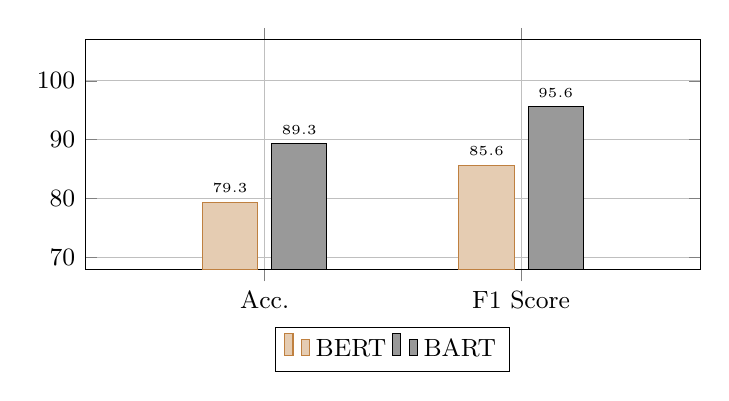
\begin{tikzpicture} 
 \begin{axis}[
 enlargelimits=0.7,
 legend style={at={(0.5,-0.25)},
  anchor=north,legend columns=-1},
 symbolic x coords={Acc., F1 Score },
 xtick=data,
 ybar=5pt,% configures `bar shift'
 bar width=20pt,
 width=9.4cm, height=4.5cm,
 nodes near coords,
 nodes near coords align={vertical},
 nodes near coords style={font=\tiny},
 font=\small,
 grid=major,
 ]
 \addplot[fill=brown!40!white,draw=brown] coordinates {
  (Acc., 79.3)
  (F1 Score, 85.6)
 };
 \addplot [fill=black!40!white,draw=black] coordinates {
  (Acc., 89.3)
  (F1 Score, 95.6)
 };
 \legend{BERT, BART}
 \end{axis}
 \end{tikzpicture}
 \caption{Performance Comparison.}
\end{figure}

\end{document}